\subsection{Convolution layer} \label{subs:2dconv}
In a \acrshort{cnn}, the \textbf{convolutional layer} carries out the feature extraction process of the input image, also called the input \acrfull{fm}. It is the main operation in a \acrshort{cnn}, and it is the layer that gives the network its name. The first layer extracts low-level features of the input \acrshort{fm} and the deepest layers use the low-level features to build high-level ones \cite{goodfellow_deep_2016}.

An input image is characterized by 3 parameters: \textbf{$N_{ix}$} the width, \textbf{$N_{iy}$} the height, and \textbf{$N_{if}$} the depth. We can illustrate then the input \acrshort{fm} as a cuboid composed of layers of pixels. An illustration is presented in Figure \ref{fig:notation:ifm}.
The convolution layer correlates therefore input \acrshort{fm} and a 4D filter, to produce output \acrshort{fm}, which contains the high-level features \cite{zhao_towards_2018}. The output \acrshort{fm} is also characterized by its width $N_{ox}$, its height $N_{oy}$ and its depth $N_{of}$. We can see a general output \acrshort{fm} in Figure \ref{fig:notation:ofm}. As a result, the filter consists of $N_{of}$ kernels, where each kernel has size $N_{kx} \times N_{ky} \times N_{if}$, that we can observe in Figure \ref{fig:notation:k}.
%
\begin{figure}
    \centering
    %
    \begin{subfigure}{.32\textwidth}
    \centering
    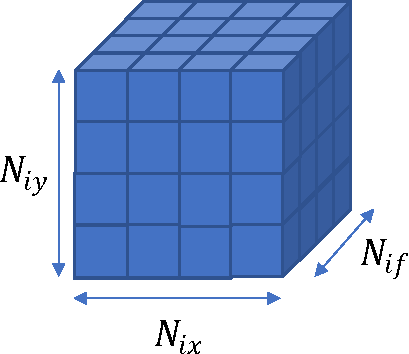
\includegraphics[width=\linewidth]{notifm.pdf}
    \caption{Input \acrshort{fm}}
    \label{fig:notation:ifm}
    \end{subfigure}
    %
    \begin{subfigure}{.32\textwidth}
    \centering
    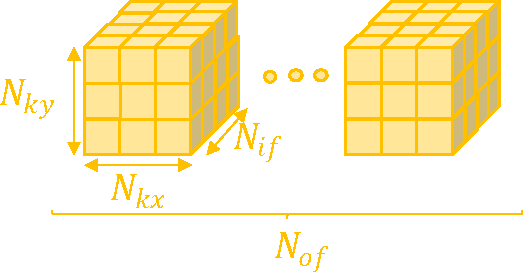
\includegraphics[width=\linewidth]{notk.pdf}
    \caption{A convolution kernel}
    \label{fig:notation:k}
    \end{subfigure}
    %
    \begin{subfigure}{.32\textwidth}
    \centering
    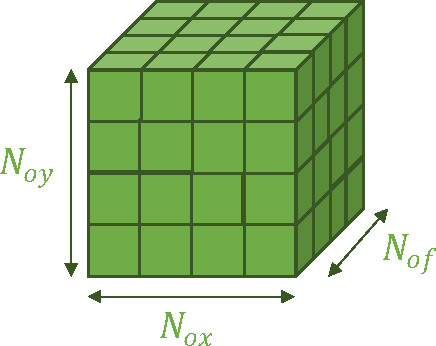
\includegraphics[width=\linewidth]{notofm.pdf}
    \caption{Output \acrshort{fm}}
    \label{fig:notation:ofm}
    \end{subfigure}
    %
    \caption{Volumes involved in the convolution operations}
    \label{fig:notconv}
\end{figure}

Convolution is a specialized kind of linear operation. The convolution operation happens as follows. Each kernel acts like a sliding window on the input \acrshort{fm}. We extract a chunk of pixels of the same size of the kernel in the input \acrshort{fm} and perform an element-wise multiplication with the chunk of data and the kernel. We sum up the computed pixels to obtain one output pixel. Sliding this kernel on the input \acrshort{fm} will produce a channel of the output \acrshort{fm}, where the output pixel at position $(x, y)$ corresponds to the movement of the sliding window from the top left of the input \acrshort{fm}. Since one kernel produces one channel of the output \acrshort{fm}, having $N_{of}$ kernels produces then $N_{of}$ channels. An illustration of the convolution operation is in Figure \ref{fig:convolution}.
%
\begin{figure}
    \centering
    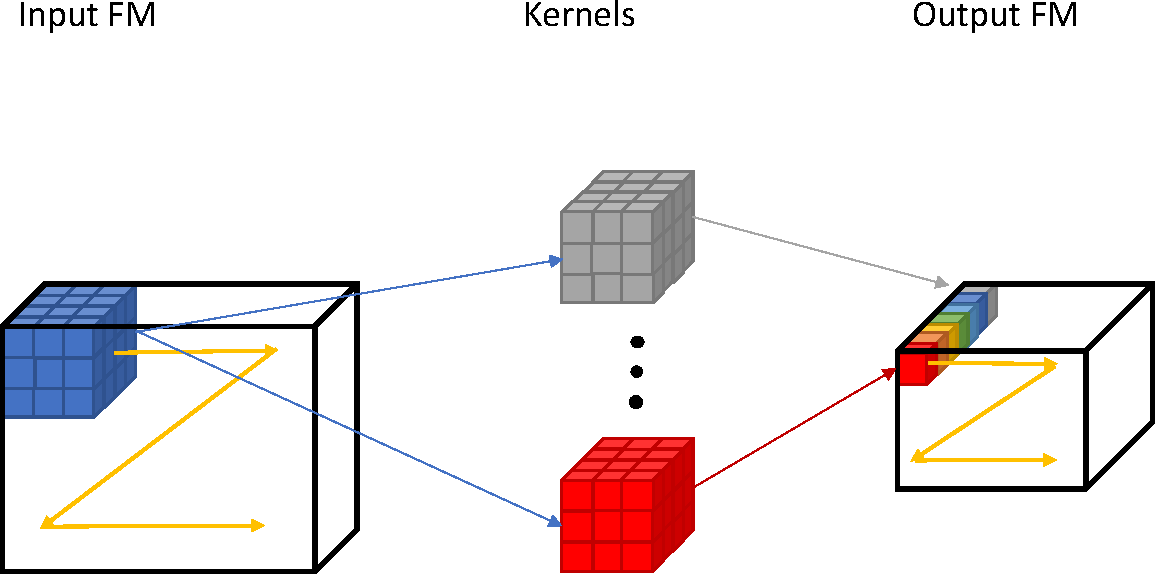
\includegraphics[width=\textwidth]{conv.pdf}
    \caption{Convolution operation}
    \label{fig:convolution}
\end{figure}

Except for $1 \times 1$ kernel, there is a spatial reduction between the input and output \acrshort{fm}s, while there is an increase in the number of channels. It is explain by the fact that the sliding window movements can not go beyond the size of the input \acrshort{fm}. We can express the spatial reduction using Equation \eqref{label:conv_spatial_red}.
%
\begin{equation}
    N_{o\{x,y\}} = N_{i\{x,y\}} - N_{k\{x,y\}} + 1
    \label{label:conv_spatial_red}
\end{equation}
%
However, we can keep the same dimensions using \textit{padding} on the boundary. It means that we pad the edges with extra pixels (usually of value 0).

Moreover, each time the sliding window performs a convolution, it shifts in the input \acrshort{fm}. The amount, by which the filter shifts, is called the \textit{stride} and it is initially set to 1. If we increase the stride, we can reduce the spatial dimensions of the output \acrshort{fm}. For example, if we use padding and a stride of 2, $\frac{N_{ix}}{N_{ox}} = \frac{N_{iy}}{N_{oy}} = \frac{1}{2}$, and the output \acrshort{fm} has 4 times fewer pixels. If we add the stride to Equation \eqref{label:conv_spatial_red}, we obtain Equation \eqref{label:conv_spatial_red_tot}, which describes the spatial reduction when performing a convolution. In Section \ref{subs:pooling}, we introduce a new layer than can also reduce the spatial dimensions of the output \acrshort{fm}.
%
\begin{equation}
    N_{o\{x,y\}} = \lfloor \frac{ N_{i\{x,y\}}}{S} \rfloor - N_{k\{x,y\}} + 1
    \label{label:conv_spatial_red_tot}
\end{equation}

Finally, we can express the convolution operations mathematically, as in Equation \eqref{eq:conv}.
%
{ \scriptsize
\begin{equation}
    \begin{split}
        & \forall ox \in \{ 1, ..., N_{ox} \}, oy \in \{ 1, ..., N_{oy} \}, of \in \{ 1, ..., N_{of} \} : \\
        & FM_O[ox, oy, oc] = \sum^{N_{if}}_{if=1}
        \sum^{N_{kx}}_{kx=1}
        \sum^{N_{ky}}_{ky=1}
        FM_I[ox \cdot S + kx - \lfloor \frac{N_{kx}}{2} \rfloor,  oy \cdot S + ky - \lfloor \frac{N_{ky}}{2} \rfloor, if] \cdot
        W^{of}_{if}[kx, ky]
    \end{split}
    \label{eq:conv}
\end{equation}
}

According to \textcite{goodfellow_deep_2016}, the convolutional layer has several advantages compared to the fully-connected layer. The convolutional layer is sparsely connected, which means that there are less connections between layers. The convolutional layer is then easier to train and the convolution keeps spatial information. It has also parameter sharing: we use the same kernel to compute one channel of the output \acrshort{fm} and the convolutional layer use fewer parameters. To illustrate this weight reduction, in AlexNet \cite{krizhevsky_imagenet_2012}, 94\% of the weights are used in the fully-connected layers. But as said earlier, convolution is a computationally heavy operation. For example, in VGG-11, 98.2\% of the operations are done in the convolution layers \cite{guo_survey_2018}. Furthermore, if the input \acrshort{fm} is a vector ($N_{ix} = N_{iy} = 1$), then it means that the convolution and the fully-connected layer perform the same operation.

As the convolution has a huge arithmetic complexity, we see in the following Section \ref{subs:dsc} an alternate way to perform convolution to reduce this.
